\documentclass[a4paper,notumble]{leaflet} %nocombine, wenns mehr als 6 Seiten werden
\usepackage[T1]{fontenc}
\usepackage[utf8]{inputenc} %alternativ latin1
\usepackage[USenglish]{babel} %übersetzt die automatisch generierten Dokumentelemente
\usepackage{listings}
\usepackage{cclicenses}
\usepackage{tikz}
\usetikzlibrary{shapes.arrows}
\usepackage{hyperref}
\usepackage{caption} %to use command \caption* without numbering
\pagenumbering{gobble}

\usepackage{pagecolor}
\definecolor{solarized_base03}{HTML}{002b36}
\definecolor{solarized_base1}{HTML}{93a1a1}
\thepagecolor=LightGoldenrod1
% \pagecolor{solarized_base03}
% \color{solarized_base1}

%%%%%%%%%%%%%%%%%%%%%%%%%%%%%%%%%%%%%%%%%%%%%%%%%%%%%%%%%%%%%%%55
\begin{document}
\author{} %suppress on maketitle
\date{\theyear}  %suppress on maketitle
\title{Git Cheat Sheet}
% Uncomment to create title page and/or toc:
%\maketitle
%\tableofcontents
\section{{\LARGE Git Cheat Sheet}}
\begin{scriptsize}
based on \textbf{Pro Git} by Scott Chacon: \url{http://git-scm.com/book}

\copyright{} \the\year{} http://steffiland.de

\href{http://creativecommons.org/licenses/by-nc-sa/3.0/}{\byncsa} This work is licensed under a Creative Commons Attribution-NonCommercial-ShareAlike 3.0 Unported License.
\end{scriptsize}
%%%%%%%%%%%%%%%%%%%%%%%%%%%%%%%%%%%%%%%%%%%%%%%%%%%%%%%%%%%%%%%%%
\section{General Setup with \texttt{git config}}
\begin{description}
\item[Usage] \verb!git config [--system|--global] <options>! operate system-wide, user-specific or just for current project
\item[view settings:] \verb!--list | -l!
\item[add a setting:] \verb!--add <key> <value>!
\item[delete a setting:] \verb!--unset <key>!
\item[setting identity:] with \verb|git config| \dots\\
	\dots \, \verb|--global user.name "John Doe"| \\
	\dots \, \verb|--global user.email johndoe@example.com|
\item[git through proxy:] \verb!--add http.proxy!
	\verb! http://wwwproxy.my.com:8080!
\end{description}

\section{Getting Help}
\verb!git help <verb> | git <verb> --help!
\verb!man git-<verb>!

\section{Getting a Git Repository}
the leading word \verb!git! will be ommitted for all commands.
\begin{description}
\item[initialize a new repo in an existing directory:] standing in the directory, run \verb!init! and add relevant files, e.g. \verb!add *.c! and \verb!commit -m 'initial project version'!
\item[create a working copy:] %
	\verb!clone <url> [<name_of_new_dir>]!; while \texttt{<url>} is sth. like \verb!git://github.com/what/ever.git! or \verb!http[s]://...! or \verb!user@server:/path.git!
\end{description}

\section{Recording Changes}
\begin{figure}[htbp]\centering
	%\includegraphics[width=\linewidth]{git}
	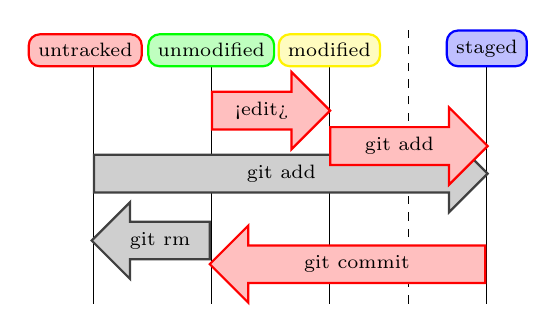
\begin{tikzpicture}[outline/.style={draw=#1,thick,fill=#1!25}]
	\draw (0,0) -- (0,3) node[above,outline=red,rounded corners,xshift=-1mm] {{\scriptsize untracked}};
	\draw (1.5,0) -- (1.5,3) node[above,outline=green,rounded corners] {{\scriptsize unmodified}};
	\draw (3,0) -- (3,3) node[above,outline=yellow,rounded corners] {{\scriptsize modified}};
	\draw[dashed,very thin] (4,0) -- (4,3.5);
	\draw (5,0) -- (5,3) node[above,outline=blue,rounded corners] {{\scriptsize staged}};
	\node[minimum height=5cm,single arrow,outline=darkgray] at (0.64+1.75,1.65) {\scriptsize git add};
	\node[minimum height=1.5cm,single arrow,outline=darkgray,shape border rotate=180] at (0.85,0.8) {\scriptsize git rm};
	\node[minimum height=1.5cm,single arrow,outline=red] at (0.64+1.5,2.45) {\scriptsize <edit>};
	\node[minimum height=2cm,single arrow,outline=red] at (0.64+3.25,2) {\scriptsize git add};
	\node[minimum height=3.5cm,single arrow,outline=red,shape border rotate=180] at (0.85+2.5,0.5) {\scriptsize git commit};
\end{tikzpicture}
	\caption*{file status lifecycle in a local repository}
\end{figure}
\begin{description}
\item[check status:] \verb!status! -- lists all untracked files, modified files (in section "Changed but not updated") and staged files (in section "Changes to be committed"). No output means that all files are unmodified.
\item[track new files:] \verb!add <file>! -- the file will now be tracked and the current version is going to be staged. If you edit this file again after doing \verb!add! and before doing \verb!commit!, the version of the file at the time you ran \verb!add! is what will be in the historical snapshot. If this is not what you want you have to rerun \verb!add!.
\item[prepare modified files for commit:] \verb!add [<file>]! -- stages the current version of the given file (or all modified files that are not excluded by \verb!.gitignore!).
\item[protect files from being tracked:] \textbf{or auto\-ma\-ti\-cally added:} Prepare a \verb!.gitignore! file with a content similar to the following:
\end{description}
\begin{lstlisting}[language=bash,frame=single,breaklines=true,breakautoindent=true,basicstyle=\ttfamily\small,fontadjust=true,prebreak={\mbox{$\hookleftarrow$}}]
# a comment this is ignored
*.a	# no .a files
!lib.a	# but do track lib.a
/TODO	# ignore the root TODO file (not subdir/TODO)
build/	# ignore all files in the build/ directory
doc/*.txt # ignore doc/notes.txt, but not doc/server/arch.txt
\end{lstlisting}
\begin{description}
\item[view modifications in detail:] \verb!diff [<file>]! -- shows what you’ve changed but not yet staged (compares working directory vs. staging area). \\
	\verb!diff --cached [<file>]! -- shows what you’ve staged (that will go into your next commit).
\item[commit staged changes:] \verb!commit [-m "message"]!
\item[commit all changes:] \verb!commit -a [-m "message"]! -- automatically stages every [already tracked] file, letting you skip the \verb!git add! part.
\item[delete a file:] \verb!rm <file>! -- deletes the file from working directory and from staging area. You have to \verb!commit! the removal. To keep the file untracked in your working copy, do \verb!rm --cached!
\item[move/rename a file:] \verb!git mv <oldfile> <newfile>! works the same way like 
\begin{lstlisting}[language=bash,breaklines=true,breakautoindent=false,basicstyle=\ttfamily\small,fontadjust=true]
mv <old> <new>
git rm <old>; git add <new>
\end{lstlisting}because Git figures out that this is a rename implicitly.
\item[Filename Globbing:] \verb!log/\*.log! matches all files that have the \verb!.log! extension in the \verb!log/! directory. The backslash in front of the \verb!*! is necessary because Git does its
own filename expansion.
\end{description}

\section{Viewing the Commit History}
\verb!git log! shows commit logs (most recent first) with checksum, author’s name and e-mail, date and commit message. The most important options are:
\begin{description}
\item[show with diffs:] \verb!-p!
\item[show newest \textit{n} commits:] \texttt{-\textit{n}} or \texttt{-n\textit{n}}
\item[show abbreviated stats for each commit:] \verb!--stat|--shortstat! -- prints a list of modified files, how many files were changed, and how many lines were added/removed for each commit. It also puts a summary of the information at the end.
\item[pretty log output:] \verb!--pretty=<style>! -- possible styles are \verb!oneline!, \verb!short!, \verb!full!, \verb!fuller! and \verb!format:"formatstring"! (see help). \verb!--graph! adds a nice little ASCII graph showing your branch and merge history.
\item[limit shown timerange:] \verb!--since|--after|! \verb!--until|--before=<date>! where the date can be specific as in \verb!2008–01–15! or relative as in \verb!2.years.1.day.3.minutes!.
\end{description}

\section{Undoing Things}
\begin{description}
\item[change last commit:] \verb!commit --amend! -- takes your staging area and uses it for changing the last commit (useful for adding forgotten files or changing the commit message).
\item[unstage a staged file:] \verb!reset HEAD <file>!
\item[revert a modified file:] \verb!checkout -- <file>!
\end{description}

\section{Working with Remote Repositories}
\begin{description}
\item[list all remote places/aliases:] \verb!remote [-v]!
\item[add remote repository alias:] \verb!remote add <rname> <url>! -- adds \verb!<url>! to be accessible via the short name \verb!<rname>! 
\item[inspect a remote:] \verb! remote show <rname>!\item[mirror remote changes to local repo copy:] \verb!fetch <rname>!
\item[fetch and merge remote to local:] \verb!pull <rname>! -- this fetches data from the server you originally cloned from and automatically tries to merge it into the code you’re currently working on.
\item[push to remote:] \texttt{push <rname> [<local\-branch>[:<remote\-branch]] [<tagname>|----tags]}, Only the \texttt{master} branch, and branches created from an remote branch, will be pushed automatically. Tags are not pushed by default.
\item[rename a remote:] \texttt{remote rename <oldrname> <newrname>} -- this changes your remote branch names, too.
\item[remove a remote reference/alias:] \verb!remote rm <rname>!
\end{description}

\section{Tagging specific points in history}
\begin{description}
\item[list available tags:] \verb!tag [-l] [<pattern>]! -- lists all tags in alphabetical order or only those matching a pattern.
\item[tag types:] A lightweight tag is just a pointer to a specific commit. Annotated tags are stored as full objects in the Git database. They’re checksummed; contain the tagger name, e-mai, and date; have a tagging message; and can be GPG-signed.
\item[create a tag:] \texttt{tag [-a|-s] <tagname> [-m <tag\-message>] [<cksum>]} -- use \verb!-a! for annotated tags or \verb!-s! for annotated and signed tags. Don't supply \verb!-m!, \verb!-a! or \verb!-s! for lightweight tags. To tag an older commit, apply (part of its) checksum at the end.
\item[show tag information:] \verb!show <tagname>!
\item[verify a signed tag:] \verb!git tag -v <tagname>!
\end{description}

\section{Tips and Tricks}
\begin{description}
\item[Shell completion:] Take the \texttt{git-com\-ple\-tion.bash} file from the Git source code and source it in your \verb!.bashrc!. The Windows Git Bash has auto-completion preconfigured.
\item[Command Aliases] can be defined via \texttt{git config ----global alias.<alias> <command>}. The command can be sth. like \texttt{checkout}, \texttt{'reset HEAD ----'} etc.
\end{description}

\section{Branches}
A branch is a lightweight movable pointer to a commit. \texttt{HEAD} is a special pointer to the branch you're currently on. Usually this is the default branch \texttt{master}. The current branch always points to the last commit you made.
\begin{description}
\item[create new branch:] \verb!branch <bname>! -- the newly created branch points to your last commit
\item[switch to another branch:] \texttt{checkout <bname>} -- changes \texttt{HEAD} and the files in your working directory appropriately.
\item[create new branch and switch to it:] \texttt{checkout -b <bname> [<basebranch>]} -- You can let start the new branch at another base than the current branch (e.g., a remote branch).
\item[merge branches:] First, switch to the branch you want to merge into (the branch that is going to be changed by the merge). Then run \texttt{git merge <bname>}. If no conflicts occur, Git automatically creates a new commit object that contains the merged work, and moves the current branch to point on it.
\item[delete an obsolete branch:] \texttt{branch -d|-D <bname>} -- \verb!-D! is a force-deletion for branches with unmerged work.
\item[show and clean merge conflicts:] Show conflicts with \texttt{git status} and clean up the files manually; then mark them as resolved using \texttt{git add}. Alternatively, use \texttt{git mergetool}, which fires up an appropriate visual merge tool and walks you through the conflicts. Finally you have to \texttt{commit} all these changes.
\item[see last commit on each branch:] \verb!git branch -v!
\item[show branches already merged into the current:] \verb!branch --merged! -- Branches listed without an $*$ can be deleted safely.
\item[show all branches with unmerged work:] \verb!branch --no-merged! -- these branches cannot be deleted with \verb!-d!, you'll have to use \verb!-D!.
\item[access branches on remote sites:] use \texttt{<rname>/<bname>}. After a \texttt{git fetch <rname>}, this will point to the current remote changes.
\item[delete a remote branch:] \texttt{push <rname> :<bname>}
\item[rebasing a branch:] \texttt{rebase <otherbranch>} -- This means to take all the changes that were committed on the current branch (after the common start of both branches) and replay them onto the other one. The current branch will point to that new state afterwards. After that you can switch to the other branch and do a fast-forward merge. \textbf{Do not rebase commits that you have pushed to a public repository!}
\end{description}
\end{document}
